\documentclass[11pt]{article}

\newcommand{\yourname}{Kevin Zhang}

\def\comments{0}

%format and packages

%\usepackage{algorithm, algorithmic}
\usepackage{forest}
\usepackage{tikz}
\usepackage{algpseudocode}
\usepackage{amsmath, amssymb, amsthm}
\usepackage{tcolorbox}
\usepackage{enumerate}
\usepackage{enumitem}
\usepackage{framed}
\usepackage{verbatim}
\usepackage[margin=1.0in]{geometry}
\usepackage{microtype}
\usepackage{kpfonts}
\usepackage{palatino}
	\DeclareMathAlphabet{\mathtt}{OT1}{cmtt}{m}{n}
	\SetMathAlphabet{\mathtt}{bold}{OT1}{cmtt}{bx}{n}
	\DeclareMathAlphabet{\mathsf}{OT1}{cmss}{m}{n}
	\SetMathAlphabet{\mathsf}{bold}{OT1}{cmss}{bx}{n}
	\renewcommand*\ttdefault{cmtt}
	\renewcommand*\sfdefault{cmss}
	\renewcommand{\baselinestretch}{1.06}

\usepackage[boxruled,vlined,nofillcomment]{algorithm2e}
	\SetKwProg{Fn}{Function}{\string:}{}
	\SetKwFor{While}{While}{}{}
	\SetKwFor{For}{For}{}{}
	\SetKwIF{If}{ElseIf}{Else}{If}{:}{ElseIf}{Else}{:}
	\SetKw{Return}{Return}
	

%enclosure macros
\newcommand{\paren}[1]{\ensuremath{\left( {#1} \right)}}
\newcommand{\bracket}[1]{\ensuremath{\left\{ {#1} \right\}}}
\renewcommand{\sb}[1]{\ensuremath{\left[ {#1} \right\]}}
\newcommand{\ab}[1]{\ensuremath{\left\langle {#1} \right\rangle}}

%probability macros
\newcommand{\ex}[2]{{\ifx&#1& \mathbb{E} \else \underset{#1}{\mathbb{E}} \fi \left[#2\right]}}
\newcommand{\pr}[2]{{\ifx&#1& \mathbb{P} \else \underset{#1}{\mathbb{P}} \fi \left[#2\right]}}
\newcommand{\var}[2]{{\ifx&#1& \mathrm{Var} \else \underset{#1}{\mathrm{Var}} \fi \left[#2\right]}}

%useful CS macros
\newcommand{\poly}{\mathrm{poly}}
\newcommand{\polylog}{\mathrm{polylog}}
\newcommand{\zo}{\{0,1\}}
\newcommand{\pmo}{\{\pm1\}}
\newcommand{\getsr}{\gets_{\mbox{\tiny R}}}
\newcommand{\card}[1]{\left| #1 \right|}
\newcommand{\set}[1]{\left\{#1\right\}}
\newcommand{\negl}{\mathrm{negl}}
\newcommand{\eps}{\varepsilon}
\DeclareMathOperator*{\argmin}{arg\,min}
\DeclareMathOperator*{\argmax}{arg\,max}
\newcommand{\eqand}{\qquad \textrm{and} \qquad}
\newcommand{\ind}[1]{\mathbb{I}\{#1\}}
\newcommand{\sslash}{\ensuremath{\mathbin{/\mkern-3mu/}}}
\newcommand{\pipe}{\hspace{3pt}|\hspace{3pt}}

%mathbb
\newcommand{\N}{\mathbb{N}}
\newcommand{\R}{\mathbb{R}}
\newcommand{\Z}{\mathbb{Z}}
%mathcal
\newcommand{\cA}{\mathcal{A}}
\newcommand{\cB}{\mathcal{B}}
\newcommand{\cC}{\mathcal{C}}
\newcommand{\cD}{\mathcal{D}}
\newcommand{\cE}{\mathcal{E}}
\newcommand{\cF}{\mathcal{F}}
\newcommand{\cL}{\mathcal{L}}
\newcommand{\cM}{\mathcal{M}}
\newcommand{\cO}{\mathcal{O}}
\newcommand{\cP}{\mathcal{P}}
\newcommand{\cQ}{\mathcal{Q}}
\newcommand{\cR}{\mathcal{R}}
\newcommand{\cS}{\mathcal{S}}
\newcommand{\cU}{\mathcal{U}}
\newcommand{\cV}{\mathcal{V}}
\newcommand{\cW}{\mathcal{W}}
\newcommand{\cX}{\mathcal{X}}
\newcommand{\cY}{\mathcal{Y}}
\newcommand{\cZ}{\mathcal{Z}}

%theorem macros
\newtheorem{thm}{Theorem}
\newtheorem{lem}[thm]{Lemma}
\newtheorem{fact}[thm]{Fact}
\newtheorem{clm}[thm]{Claim}
\newtheorem{rem}[thm]{Remark}
\newtheorem{coro}[thm]{Corollary}
\newtheorem{prop}[thm]{Proposition}
\newtheorem{conj}[thm]{Conjecture}

\theoremstyle{definition}
\newtheorem{defn}[thm]{Definition}
\newtheoremstyle{case}{}{}{}{}{}{:}{ }{}
\theoremstyle{case}
\newtheorem{case}{Case}

\theoremstyle{theorem}
\newtheorem{prob}{Problem}
\newtheorem{sol}{Solution}

\tikzset{every picture/.style={line width=0.75pt}} %set default line width to 0.75pt        

\begin{document}
{\large
\noindent Name: \yourname}

\vspace{15pt}

\begin{prob}\end{prob}

\begin{enumerate}[label=(\alph*)]

\item
$aabaab$ is not in $L(G)$. The reason is that there is no way to have a $b$ at the end on its own.
The only derivation that results in a $b$ is $B \rightarrow bA$, and since there is no derivation
$A \rightarrow \varepsilon$, there is no way to have $b$ at the end.

\item
$aaaaba$ is in $L(G)$. The derivation is as follows
\begin{flalign*}
S &\rightarrow AB & \\
  &\rightarrow aAB  \\
  &\rightarrow aAbA \\
  &\rightarrow aAba \\
  &\rightarrow aaAba\\
  &\rightarrow aaaAba\\
  &\rightarrow aaaaba
\end{flalign*}

\item
$aabbaa$ is not in $L(G)$. The same reasoning for $(a)$ applies. It is not possible to have the two
$b$'s together in the center, without any $a$s, because the only derivation that results in a $b$
is $B \rightarrow bA$. Since $A \rightarrow \varepsilon$ is not possible, there must be at least one
$a$ between $b$'s

\item
$abaaba$ is in $L(G)$. The derivation is as follows
\begin{flalign*}
S &\rightarrow ABS & \\
  &\rightarrow ABAB \\
  &\rightarrow aBaB \\
  &\rightarrow abAabA \\
  &\rightarrow abaaba
\end{flalign*}

\end{enumerate}

\newpage

\begin{prob}\end{prob}

\begin{enumerate}[label=(\alph*)]

\item
Derivation:
\begin{flalign*}
E &\rightarrow T & \\
  &\rightarrow F \\
  &\rightarrow a
\end{flalign*}

Parse Tree:

\begin{forest}
[E [T [F [\textit{a}]]]]
\end{forest}

\item
Derivation:
\begin{flalign*}
E &\rightarrow E + T & \\
  &\rightarrow E + T + T \\
  &\rightarrow T + T + T \\
  &\rightarrow F + F + F \\
  &\rightarrow a + a + a
\end{flalign*}

Parse Tree:

\begin{forest}
[E 
  [E 
   [E [T [F [\textit{a}]]]] 
   [+] 
   [T [F [\textit{a}]]]
  ]
  [+]
  [T [F [\textit{a}]]]
]
\end{forest}

\newpage

\item
Derivation:
\begin{flalign*}
E &\rightarrow T & \\
  &\rightarrow F  \\
  &\rightarrow (E) \\
  &\rightarrow (T) \\
  &\rightarrow (F) \\
  &\rightarrow ((E)) \\
  &\rightarrow ((T)) \\
  &\rightarrow ((F)) \\
  &\rightarrow ((a))
\end{flalign*}

Parse Tree:

\begin{forest}
[E [T [F [(] 
         [E [T [F [(]
                  [E [T [F [a]]]]
                  [)]]]] 
         [)] ]]]
\end{forest}

\end{enumerate}

\newpage

\begin{prob}\end{prob}

\begin{enumerate}[label=(\alph*)]

\item
\begin{flalign*}
S &\rightarrow aB & \\
  &\rightarrow aaBB \\
  &\rightarrow aabSB \\
  &\rightarrow aabB \\
  &\rightarrow aabbS \\
  &\rightarrow aabb \\
\end{flalign*}

\item
\begin{flalign*}
S &\rightarrow aB & \\
  &\rightarrow aaBB \\
  &\rightarrow aaBaBB \\
  &\rightarrow aaBaBbS \\
  &\rightarrow aaBaBb \\
  &\rightarrow aaBabSb \\
  &\rightarrow aaBabb \\
  &\rightarrow aabSabb \\
  &\rightarrow aababb \\
\end{flalign*}

\item

\hspace{1px}\\

\begin{forest}
[S 
 [\textit{a}]
 [B 
  [\textit{b}]
  [S 
   [\textit{b}]
   [A 
    [\textit{a}]
    [S [$\varepsilon$]]
   ]
  ]
 ]
]  
\end{forest}

\end{enumerate}

\newpage

\begin{prob}\end{prob}

\begin{enumerate}[label=(\alph*)]

\item
$V = \{S\}$ \\
$\Sigma = \{a, b\}$ \\
$R = \{\}$ \\
$S = S$

\item
$V = \{S\}$ \\
$\Sigma = \{a, b\}$ \\
$R = \{
S \rightarrow a \pipe b \pipe aaS \pipe abS \pipe baS \pipe bbS
\}$ \\
$S = S$

\item
$V = \{S\}$ \\
$\Sigma = \{a, b\}$ \\
$R = \{
S \rightarrow \varepsilon \pipe Sb \pipe aSb
\}$ \\
$S = S$

\item
$V = \{S, T\}$ \\
$\Sigma = \{a, b\}$ \\
$R = \{
S \rightarrow TaTaTaTaT, \hspace{10pt}
T \rightarrow \varepsilon \pipe aT \pipe bT 
\}$ \\
$S = S$

\item
$V = \{S, T\}$ \\
$\Sigma = \{a, b\}$ \\
$R = \{ 
S \rightarrow aTa \pipe bTb, \hspace{10pt}
T \rightarrow \varepsilon \pipe aT \pipe bT
\}$ \\
$S = S$

\end{enumerate}

\begin{prob}\end{prob}

\begin{enumerate}[label=(\alph*)]

\item
$V = \{S, T, F\}$ \\
$\Sigma = \{a, b, c\}$ \\
$R = \{
S \rightarrow TF, \hspace{10pt}
T \rightarrow \varepsilon \pipe aTb, \hspace{10pt}
F \rightarrow \varepsilon \pipe bFc
\}$ \\
$S = S$ \\
\textbf{Reasoning:} For every $a$ or $c$, we need to have a $b$. We cannot mix the 
$a$s on the left with the $c$s on the right, so we need intermediary variables
to prevent mixing, but the $b$s can be joined in the middle.

\item
$V = \{S, T\}$ \\
$\Sigma = \{a, b, c\}$ \\
$R = \{
S \rightarrow \varepsilon \pipe aSc \pipe T, \hspace{10pt}
T \rightarrow \varepsilon \pipe aTb
\}$ \\
$S = S$ \\
\textbf{Reasoning:} For every $b$ or $c$, we need to have a $a$. We can first 
fix the number of $c$s we want, and then squeeze the number of $b$s in between.
Everything, is of course, prepended with an $a$, so the counts line up.
\end{enumerate}

\newpage

\begin{prob}\end{prob}

\noindent
$V = \{S, T, F\}$ \\
$\Sigma = \{0, 1\}$ \\
$R = \{
S \rightarrow \varepsilon \pipe 0S \pipe 1T, \hspace{10pt}
T \rightarrow 0F \pipe 1S, \hspace{10pt}
F \rightarrow 1F \pipe 0T
\}$ \\
$S = S$\\
\textbf{Reasoning:} The substituions from HW2 10F translate nicely here, with each of 
$S$, $T$, $F$ representing a state. $S$ has the only terminal derviation, so all words
generated need to end in $S$.

\begin{prob}\end{prob}

\begin{enumerate}[label=(\alph*)]

\item
\textbf{Initial} \\
$S \rightarrow aSab \pipe B$ \\
$B \rightarrow bbC \pipe bb$ \\
$C \rightarrow \varepsilon \pipe cC$ \\
\textbf{Pass 1} \\
$S_{new} \rightarrow S$ \\
$S \rightarrow aSab \pipe B$ \\
$B \rightarrow bbC \pipe bb$ \\
$C \rightarrow \varepsilon \pipe cC$ \\
\textbf{Pass 2} \\
$S_{new} \rightarrow S$ \\
$S \rightarrow aSab \pipe B$ \\
$B \rightarrow bbC \pipe bb$ \\
$C \rightarrow cC$ \\
\textbf{Pass 3} \\
$S_{new} \rightarrow aSab \pipe bbC \pipe bb$ \\
$S \rightarrow aSab \pipe bbC \pipe bb$ \\
$B \rightarrow bbC \pipe bb$ \\
$C \rightarrow cC$ \\
\textbf{Pass 4} \\
$S_{new} \rightarrow aW_1 \pipe bW_3 \pipe bb$ \\
$S \rightarrow aW_1 \pipe bW_3 \pipe bb$ \\
$B \rightarrow bW_3 \pipe bb$ \\
$C \rightarrow cC$ \\
$W_1 \rightarrow SW_2$ \\
$W_2 \rightarrow ab$ \\
$W_2 \rightarrow bC$ \\
\textbf{Pass 5} \\
$S_{new} \rightarrow T_{1}W_{1} \pipe T_{b}W_{3} \pipe T_{b}T_{b}$ \\
$S \rightarrow T_{a}W_{1} \pipe T_{b}W_{3} \pipe T_{b}T_{b}$ \\
$B \rightarrow T_{b}W_{3} \pipe T_{b}T_{b}$ \\
$C \rightarrow T_{c}C$ \\
$W_1 \rightarrow SW_2$ \\
$W_2 \rightarrow T_{a}T_{b}$ \\
$W_2 \rightarrow T_{b}C$ \\
$T_a \rightarrow a$ \\
$T_b \rightarrow b$ \\
$T_c \rightarrow c$

\item
\textbf{Initial} \\
$S \rightarrow AB$ \\
$A \rightarrow a \pipe B$\\
$B \rightarrow b \pipe A \pipe \varepsilon$ \\
\textbf{Pass 1} \\
$S_{new} \rightarrow S$ \\
$S \rightarrow AB$ \\
$A \rightarrow a \pipe B$\\
$B \rightarrow b \pipe A \pipe \varepsilon$ \\
\textbf{Pass 2} \\
$S_{new} \rightarrow S \pipe \varepsilon$ \\
$S \rightarrow AB \pipe A \pipe B$ \\
$A \rightarrow a \pipe B$\\
$B \rightarrow b \pipe A$\\
\textbf{Pass 3} \\
$S_{new} \rightarrow S \pipe \varepsilon$ \\
$S \rightarrow AB \pipe A \pipe AA$ \\
$A \rightarrow a \pipe b$\\
$B \rightarrow b$\\

\end{enumerate}

\begin{prob}\end{prob}

\begin{enumerate}[label=(\alph*)]

\item



\tikzset{every picture/.style={line width=0.75pt}} %set default line width to 0.75pt        

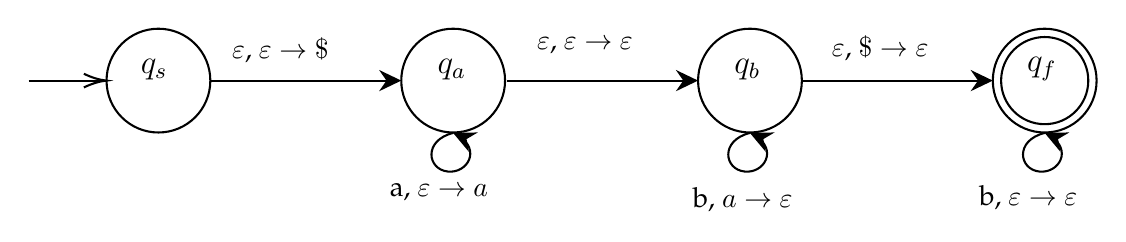
\begin{tikzpicture}[x=0.75pt,y=0.75pt,yscale=-1,xscale=1]
%uncomment if require: \path (0,126); %set diagram left start at 0, and has height of 126

%Shape: Circle [id:dp02467279464812555] 
\draw   (57,41) .. controls (57,27.19) and (68.19,16) .. (82,16) .. controls (95.81,16) and (107,27.19) .. (107,41) .. controls (107,54.81) and (95.81,66) .. (82,66) .. controls (68.19,66) and (57,54.81) .. (57,41) -- cycle ;
%Shape: Circle [id:dp08603449013351061] 
\draw   (199,41) .. controls (199,27.19) and (210.19,16) .. (224,16) .. controls (237.81,16) and (249,27.19) .. (249,41) .. controls (249,54.81) and (237.81,66) .. (224,66) .. controls (210.19,66) and (199,54.81) .. (199,41) -- cycle ;
%Straight Lines [id:da25487474417945655] 
\draw    (19.5,41) -- (55,41) ;
\draw [shift={(57,41)}, rotate = 180] [color={rgb, 255:red, 0; green, 0; blue, 0 }  ][line width=0.75]    (10.93,-3.29) .. controls (6.95,-1.4) and (3.31,-0.3) .. (0,0) .. controls (3.31,0.3) and (6.95,1.4) .. (10.93,3.29)   ;
%Straight Lines [id:da2546837432527995] 
\draw    (107,41) -- (196,41) ;
\draw [shift={(199,41)}, rotate = 180] [fill={rgb, 255:red, 0; green, 0; blue, 0 }  ][line width=0.08]  [draw opacity=0] (10.72,-5.15) -- (0,0) -- (10.72,5.15) -- (7.12,0) -- cycle    ;
%Curve Lines [id:da7758726825307602] 
\draw    (223.98,66.22) .. controls (209.48,69.82) and (211.48,83.82) .. (221.48,84.82) .. controls (230.83,85.76) and (237.56,74.45) .. (226.54,67.59) ;
\draw [shift={(223.98,66.22)}, rotate = 384.47] [fill={rgb, 255:red, 0; green, 0; blue, 0 }  ][line width=0.08]  [draw opacity=0] (10.72,-5.15) -- (0,0) -- (10.72,5.15) -- (7.12,0) -- cycle    ;
%Shape: Circle [id:dp6640176182056172] 
\draw   (342,41) .. controls (342,27.19) and (353.19,16) .. (367,16) .. controls (380.81,16) and (392,27.19) .. (392,41) .. controls (392,54.81) and (380.81,66) .. (367,66) .. controls (353.19,66) and (342,54.81) .. (342,41) -- cycle ;
%Straight Lines [id:da29958928611572033] 
\draw    (250,41) -- (339,41) ;
\draw [shift={(342,41)}, rotate = 180] [fill={rgb, 255:red, 0; green, 0; blue, 0 }  ][line width=0.08]  [draw opacity=0] (10.72,-5.15) -- (0,0) -- (10.72,5.15) -- (7.12,0) -- cycle    ;
%Curve Lines [id:da3998671188331755] 
\draw    (366.98,66.22) .. controls (352.48,69.82) and (354.48,83.82) .. (364.48,84.82) .. controls (373.83,85.76) and (380.56,74.45) .. (369.54,67.59) ;
\draw [shift={(366.98,66.22)}, rotate = 384.47] [fill={rgb, 255:red, 0; green, 0; blue, 0 }  ][line width=0.08]  [draw opacity=0] (10.72,-5.15) -- (0,0) -- (10.72,5.15) -- (7.12,0) -- cycle    ;
%Shape: Circle [id:dp7183767112344592] 
\draw   (484,41) .. controls (484,27.19) and (495.19,16) .. (509,16) .. controls (522.81,16) and (534,27.19) .. (534,41) .. controls (534,54.81) and (522.81,66) .. (509,66) .. controls (495.19,66) and (484,54.81) .. (484,41) -- cycle ;
%Straight Lines [id:da635464615439878] 
\draw    (392,41) -- (481,41) ;
\draw [shift={(484,41)}, rotate = 180] [fill={rgb, 255:red, 0; green, 0; blue, 0 }  ][line width=0.08]  [draw opacity=0] (10.72,-5.15) -- (0,0) -- (10.72,5.15) -- (7.12,0) -- cycle    ;
%Curve Lines [id:da6871537839233754] 
\draw    (508.98,66.22) .. controls (494.48,69.82) and (496.48,83.82) .. (506.48,84.82) .. controls (515.83,85.76) and (522.56,74.45) .. (511.54,67.59) ;
\draw [shift={(508.98,66.22)}, rotate = 384.47] [fill={rgb, 255:red, 0; green, 0; blue, 0 }  ][line width=0.08]  [draw opacity=0] (10.72,-5.15) -- (0,0) -- (10.72,5.15) -- (7.12,0) -- cycle    ;
%Shape: Circle [id:dp4769952887252291] 
\draw   (488,41) .. controls (488,29.4) and (497.4,20) .. (509,20) .. controls (520.6,20) and (530,29.4) .. (530,41) .. controls (530,52.6) and (520.6,62) .. (509,62) .. controls (497.4,62) and (488,52.6) .. (488,41) -- cycle ;

% Text Node
\draw (72,29) node [anchor=north west][inner sep=0.75pt]  [font=\large] [align=left] {$\displaystyle q_{s}$};
% Text Node
\draw (215,29) node [anchor=north west][inner sep=0.75pt]  [font=\large] [align=left] {$\displaystyle q_{a}$};
% Text Node
\draw (116,19) node [anchor=north west][inner sep=0.75pt]   [align=left] {$\displaystyle \varepsilon $, $\displaystyle \varepsilon \rightarrow \$$};
% Text Node
\draw (358,29) node [anchor=north west][inner sep=0.75pt]  [font=\large] [align=left] {$\displaystyle q_{b}$};
% Text Node
\draw (263,19) node [anchor=north west][inner sep=0.75pt]   [align=left] {$\displaystyle \varepsilon $, $\displaystyle \varepsilon \rightarrow \varepsilon $};
% Text Node
\draw (499,28) node [anchor=north west][inner sep=0.75pt]  [font=\large] [align=left] {$\displaystyle q_{f}$};
% Text Node
\draw (405,18) node [anchor=north west][inner sep=0.75pt]   [align=left] {$\displaystyle \varepsilon $, $\displaystyle \$\rightarrow \varepsilon $};
% Text Node
\draw (192,89) node [anchor=north west][inner sep=0.75pt]   [align=left] {a, $\displaystyle \varepsilon \rightarrow a$};
% Text Node
\draw (338,91) node [anchor=north west][inner sep=0.75pt]   [align=left] {b, $\displaystyle a\rightarrow \varepsilon $};
% Text Node
\draw (476,90) node [anchor=north west][inner sep=0.75pt]   [align=left] {b, $\displaystyle \varepsilon \rightarrow \varepsilon $};


\end{tikzpicture}


\item



\tikzset{every picture/.style={line width=0.75pt}} %set default line width to 0.75pt        

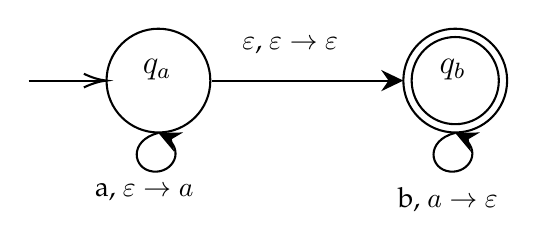
\begin{tikzpicture}[x=0.75pt,y=0.75pt,yscale=-1,xscale=1]
%uncomment if require: \path (0,122); %set diagram left start at 0, and has height of 122

%Shape: Circle [id:dp9739585981109569] 
\draw   (61,36) .. controls (61,22.19) and (72.19,11) .. (86,11) .. controls (99.81,11) and (111,22.19) .. (111,36) .. controls (111,49.81) and (99.81,61) .. (86,61) .. controls (72.19,61) and (61,49.81) .. (61,36) -- cycle ;
%Straight Lines [id:da4642773377889531] 
\draw    (23.5,36) -- (59,36) ;
\draw [shift={(61,36)}, rotate = 180] [color={rgb, 255:red, 0; green, 0; blue, 0 }  ][line width=0.75]    (10.93,-3.29) .. controls (6.95,-1.4) and (3.31,-0.3) .. (0,0) .. controls (3.31,0.3) and (6.95,1.4) .. (10.93,3.29)   ;
%Curve Lines [id:da36150169081222416] 
\draw    (85.98,61.22) .. controls (71.48,64.82) and (73.48,78.82) .. (83.48,79.82) .. controls (92.83,80.76) and (99.56,69.45) .. (88.54,62.59) ;
\draw [shift={(85.98,61.22)}, rotate = 384.47] [fill={rgb, 255:red, 0; green, 0; blue, 0 }  ][line width=0.08]  [draw opacity=0] (10.72,-5.15) -- (0,0) -- (10.72,5.15) -- (7.12,0) -- cycle    ;
%Shape: Circle [id:dp4942119055777072] 
\draw   (204,36) .. controls (204,22.19) and (215.19,11) .. (229,11) .. controls (242.81,11) and (254,22.19) .. (254,36) .. controls (254,49.81) and (242.81,61) .. (229,61) .. controls (215.19,61) and (204,49.81) .. (204,36) -- cycle ;
%Straight Lines [id:da9015186749275621] 
\draw    (112,36) -- (201,36) ;
\draw [shift={(204,36)}, rotate = 180] [fill={rgb, 255:red, 0; green, 0; blue, 0 }  ][line width=0.08]  [draw opacity=0] (10.72,-5.15) -- (0,0) -- (10.72,5.15) -- (7.12,0) -- cycle    ;
%Curve Lines [id:da07504851160669102] 
\draw    (228.98,61.22) .. controls (214.48,64.82) and (216.48,78.82) .. (226.48,79.82) .. controls (235.83,80.76) and (242.56,69.45) .. (231.54,62.59) ;
\draw [shift={(228.98,61.22)}, rotate = 384.47] [fill={rgb, 255:red, 0; green, 0; blue, 0 }  ][line width=0.08]  [draw opacity=0] (10.72,-5.15) -- (0,0) -- (10.72,5.15) -- (7.12,0) -- cycle    ;
%Shape: Circle [id:dp5563828888727453] 
\draw   (208,36) .. controls (208,24.4) and (217.4,15) .. (229,15) .. controls (240.6,15) and (250,24.4) .. (250,36) .. controls (250,47.6) and (240.6,57) .. (229,57) .. controls (217.4,57) and (208,47.6) .. (208,36) -- cycle ;

% Text Node
\draw (77,24) node [anchor=north west][inner sep=0.75pt]  [font=\large] [align=left] {$\displaystyle q_{a}$};
% Text Node
\draw (220,24) node [anchor=north west][inner sep=0.75pt]  [font=\large] [align=left] {$\displaystyle q_{b}$};
% Text Node
\draw (125,14) node [anchor=north west][inner sep=0.75pt]   [align=left] {$\displaystyle \varepsilon $, $\displaystyle \varepsilon \rightarrow \varepsilon $};
% Text Node
\draw (54,84) node [anchor=north west][inner sep=0.75pt]   [align=left] {a, $\displaystyle \varepsilon \rightarrow a$};
% Text Node
\draw (200,86) node [anchor=north west][inner sep=0.75pt]   [align=left] {b, $\displaystyle a\rightarrow \varepsilon $};


\end{tikzpicture}


\end{enumerate}

\newpage

\begin{prob}\end{prob}





\tikzset{every picture/.style={line width=0.75pt}} %set default line width to 0.75pt        

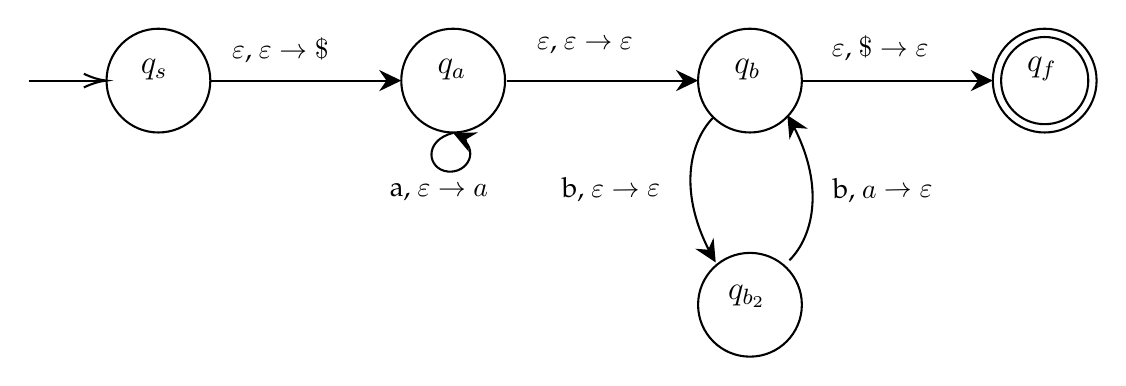
\begin{tikzpicture}[x=0.75pt,y=0.75pt,yscale=-1,xscale=1]
%uncomment if require: \path (0,190); %set diagram left start at 0, and has height of 190

%Shape: Circle [id:dp2855372048209839] 
\draw   (63,42) .. controls (63,28.19) and (74.19,17) .. (88,17) .. controls (101.81,17) and (113,28.19) .. (113,42) .. controls (113,55.81) and (101.81,67) .. (88,67) .. controls (74.19,67) and (63,55.81) .. (63,42) -- cycle ;
%Shape: Circle [id:dp5705151514591731] 
\draw   (205,42) .. controls (205,28.19) and (216.19,17) .. (230,17) .. controls (243.81,17) and (255,28.19) .. (255,42) .. controls (255,55.81) and (243.81,67) .. (230,67) .. controls (216.19,67) and (205,55.81) .. (205,42) -- cycle ;
%Straight Lines [id:da11951110025548362] 
\draw    (25.5,42) -- (61,42) ;
\draw [shift={(63,42)}, rotate = 180] [color={rgb, 255:red, 0; green, 0; blue, 0 }  ][line width=0.75]    (10.93,-3.29) .. controls (6.95,-1.4) and (3.31,-0.3) .. (0,0) .. controls (3.31,0.3) and (6.95,1.4) .. (10.93,3.29)   ;
%Straight Lines [id:da06163412487153974] 
\draw    (113,42) -- (202,42) ;
\draw [shift={(205,42)}, rotate = 180] [fill={rgb, 255:red, 0; green, 0; blue, 0 }  ][line width=0.08]  [draw opacity=0] (10.72,-5.15) -- (0,0) -- (10.72,5.15) -- (7.12,0) -- cycle    ;
%Curve Lines [id:da9539673204567258] 
\draw    (229.98,67.22) .. controls (215.48,70.82) and (217.48,84.82) .. (227.48,85.82) .. controls (236.83,86.76) and (243.56,75.45) .. (232.54,68.59) ;
\draw [shift={(229.98,67.22)}, rotate = 384.47] [fill={rgb, 255:red, 0; green, 0; blue, 0 }  ][line width=0.08]  [draw opacity=0] (10.72,-5.15) -- (0,0) -- (10.72,5.15) -- (7.12,0) -- cycle    ;
%Shape: Circle [id:dp059655303465880216] 
\draw   (348,42) .. controls (348,28.19) and (359.19,17) .. (373,17) .. controls (386.81,17) and (398,28.19) .. (398,42) .. controls (398,55.81) and (386.81,67) .. (373,67) .. controls (359.19,67) and (348,55.81) .. (348,42) -- cycle ;
%Straight Lines [id:da5482965070695474] 
\draw    (256,42) -- (345,42) ;
\draw [shift={(348,42)}, rotate = 180] [fill={rgb, 255:red, 0; green, 0; blue, 0 }  ][line width=0.08]  [draw opacity=0] (10.72,-5.15) -- (0,0) -- (10.72,5.15) -- (7.12,0) -- cycle    ;
%Shape: Circle [id:dp7039062538584582] 
\draw   (490,42) .. controls (490,28.19) and (501.19,17) .. (515,17) .. controls (528.81,17) and (540,28.19) .. (540,42) .. controls (540,55.81) and (528.81,67) .. (515,67) .. controls (501.19,67) and (490,55.81) .. (490,42) -- cycle ;
%Straight Lines [id:da7411206439245364] 
\draw    (398,42) -- (487,42) ;
\draw [shift={(490,42)}, rotate = 180] [fill={rgb, 255:red, 0; green, 0; blue, 0 }  ][line width=0.08]  [draw opacity=0] (10.72,-5.15) -- (0,0) -- (10.72,5.15) -- (7.12,0) -- cycle    ;
%Shape: Circle [id:dp5153924072944416] 
\draw   (494,42) .. controls (494,30.4) and (503.4,21) .. (515,21) .. controls (526.6,21) and (536,30.4) .. (536,42) .. controls (536,53.6) and (526.6,63) .. (515,63) .. controls (503.4,63) and (494,53.6) .. (494,42) -- cycle ;
%Shape: Circle [id:dp028443616342597622] 
\draw   (348,150) .. controls (348,136.19) and (359.19,125) .. (373,125) .. controls (386.81,125) and (398,136.19) .. (398,150) .. controls (398,163.81) and (386.81,175) .. (373,175) .. controls (359.19,175) and (348,163.81) .. (348,150) -- cycle ;
%Curve Lines [id:da4941636404938836] 
\draw    (355.5,59.6) .. controls (343.8,71.3) and (337.8,96.31) .. (355.12,127.21) ;
\draw [shift={(356.5,129.6)}, rotate = 239.3] [fill={rgb, 255:red, 0; green, 0; blue, 0 }  ][line width=0.08]  [draw opacity=0] (10.72,-5.15) -- (0,0) -- (10.72,5.15) -- (7.12,0) -- cycle    ;
%Curve Lines [id:da7490353829966909] 
\draw    (391.99,128.6) .. controls (403.69,116.9) and (409.68,91.89) .. (392.37,60.99) ;
\draw [shift={(390.99,58.6)}, rotate = 419.3] [fill={rgb, 255:red, 0; green, 0; blue, 0 }  ][line width=0.08]  [draw opacity=0] (10.72,-5.15) -- (0,0) -- (10.72,5.15) -- (7.12,0) -- cycle    ;

% Text Node
\draw (78,30) node [anchor=north west][inner sep=0.75pt]  [font=\large] [align=left] {$\displaystyle q_{s}$};
% Text Node
\draw (221,30) node [anchor=north west][inner sep=0.75pt]  [font=\large] [align=left] {$\displaystyle q_{a}$};
% Text Node
\draw (122,20) node [anchor=north west][inner sep=0.75pt]   [align=left] {$\displaystyle \varepsilon $, $\displaystyle \varepsilon \rightarrow \$$};
% Text Node
\draw (364,30) node [anchor=north west][inner sep=0.75pt]  [font=\large] [align=left] {$\displaystyle q_{b}$};
% Text Node
\draw (269,20) node [anchor=north west][inner sep=0.75pt]   [align=left] {$\displaystyle \varepsilon $, $\displaystyle \varepsilon \rightarrow \varepsilon $};
% Text Node
\draw (505,29) node [anchor=north west][inner sep=0.75pt]  [font=\large] [align=left] {$\displaystyle q_{f}$};
% Text Node
\draw (411,19) node [anchor=north west][inner sep=0.75pt]   [align=left] {$\displaystyle \varepsilon $, $\displaystyle \$\rightarrow \varepsilon $};
% Text Node
\draw (198,90) node [anchor=north west][inner sep=0.75pt]   [align=left] {a, $\displaystyle \varepsilon \rightarrow a$};
% Text Node
\draw (280.89,87.35) node [anchor=north west][inner sep=0.75pt]  [rotate=-359.31] [align=left] {b, $\displaystyle \varepsilon \rightarrow \varepsilon $};
% Text Node
\draw (361,139) node [anchor=north west][inner sep=0.75pt]  [font=\large] [align=left] {$\displaystyle q_{b_{2}}$};
% Text Node
\draw (411.29,87.86) node [anchor=north west][inner sep=0.75pt]  [rotate=-358.7] [align=left] {b, $\displaystyle a\rightarrow \varepsilon $};


\end{tikzpicture}


Here, $q_s$ is the start state. $q_a$ is a state in which we are counting the number of $a$s 
(by pushing onto the stack). $q_b$ and $q_{b_2}$ are states to ensure we read 2 $b$s for every
$a$ we are popping off the stack. $q_f$ is a final accepting state, to ensure that we don't have
anything more to read.

\begin{prob}\end{prob}



\tikzset{every picture/.style={line width=0.75pt}} %set default line width to 0.75pt        

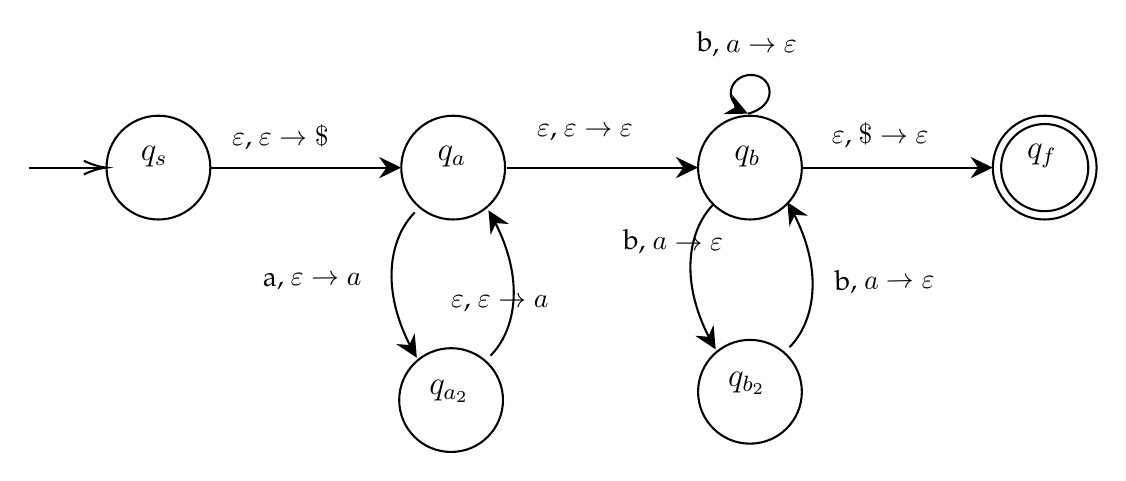
\begin{tikzpicture}[x=0.75pt,y=0.75pt,yscale=-1,xscale=1]
%uncomment if require: \path (0,255); %set diagram left start at 0, and has height of 255

%Shape: Circle [id:dp31095782904633973] 
\draw   (58,88) .. controls (58,74.19) and (69.19,63) .. (83,63) .. controls (96.81,63) and (108,74.19) .. (108,88) .. controls (108,101.81) and (96.81,113) .. (83,113) .. controls (69.19,113) and (58,101.81) .. (58,88) -- cycle ;
%Shape: Circle [id:dp9775615855572408] 
\draw   (200,88) .. controls (200,74.19) and (211.19,63) .. (225,63) .. controls (238.81,63) and (250,74.19) .. (250,88) .. controls (250,101.81) and (238.81,113) .. (225,113) .. controls (211.19,113) and (200,101.81) .. (200,88) -- cycle ;
%Straight Lines [id:da5890745087933444] 
\draw    (20.5,88) -- (56,88) ;
\draw [shift={(58,88)}, rotate = 180] [color={rgb, 255:red, 0; green, 0; blue, 0 }  ][line width=0.75]    (10.93,-3.29) .. controls (6.95,-1.4) and (3.31,-0.3) .. (0,0) .. controls (3.31,0.3) and (6.95,1.4) .. (10.93,3.29)   ;
%Straight Lines [id:da336889532719834] 
\draw    (108,88) -- (197,88) ;
\draw [shift={(200,88)}, rotate = 180] [fill={rgb, 255:red, 0; green, 0; blue, 0 }  ][line width=0.08]  [draw opacity=0] (10.72,-5.15) -- (0,0) -- (10.72,5.15) -- (7.12,0) -- cycle    ;
%Shape: Circle [id:dp2234991869088474] 
\draw   (343,88) .. controls (343,74.19) and (354.19,63) .. (368,63) .. controls (381.81,63) and (393,74.19) .. (393,88) .. controls (393,101.81) and (381.81,113) .. (368,113) .. controls (354.19,113) and (343,101.81) .. (343,88) -- cycle ;
%Straight Lines [id:da688705321071774] 
\draw    (251,88) -- (340,88) ;
\draw [shift={(343,88)}, rotate = 180] [fill={rgb, 255:red, 0; green, 0; blue, 0 }  ][line width=0.08]  [draw opacity=0] (10.72,-5.15) -- (0,0) -- (10.72,5.15) -- (7.12,0) -- cycle    ;
%Shape: Circle [id:dp4722043208819764] 
\draw   (485,88) .. controls (485,74.19) and (496.19,63) .. (510,63) .. controls (523.81,63) and (535,74.19) .. (535,88) .. controls (535,101.81) and (523.81,113) .. (510,113) .. controls (496.19,113) and (485,101.81) .. (485,88) -- cycle ;
%Straight Lines [id:da5377319161856686] 
\draw    (393,88) -- (482,88) ;
\draw [shift={(485,88)}, rotate = 180] [fill={rgb, 255:red, 0; green, 0; blue, 0 }  ][line width=0.08]  [draw opacity=0] (10.72,-5.15) -- (0,0) -- (10.72,5.15) -- (7.12,0) -- cycle    ;
%Shape: Circle [id:dp19502875239358541] 
\draw   (489,88) .. controls (489,76.4) and (498.4,67) .. (510,67) .. controls (521.6,67) and (531,76.4) .. (531,88) .. controls (531,99.6) and (521.6,109) .. (510,109) .. controls (498.4,109) and (489,99.6) .. (489,88) -- cycle ;
%Shape: Circle [id:dp7422765522499128] 
\draw   (343,196) .. controls (343,182.19) and (354.19,171) .. (368,171) .. controls (381.81,171) and (393,182.19) .. (393,196) .. controls (393,209.81) and (381.81,221) .. (368,221) .. controls (354.19,221) and (343,209.81) .. (343,196) -- cycle ;
%Curve Lines [id:da6310812450946914] 
\draw    (350.5,105.6) .. controls (338.8,117.3) and (332.8,142.31) .. (350.12,173.21) ;
\draw [shift={(351.5,175.6)}, rotate = 239.3] [fill={rgb, 255:red, 0; green, 0; blue, 0 }  ][line width=0.08]  [draw opacity=0] (10.72,-5.15) -- (0,0) -- (10.72,5.15) -- (7.12,0) -- cycle    ;
%Curve Lines [id:da2559080561775531] 
\draw    (386.99,174.6) .. controls (398.69,162.9) and (404.68,137.89) .. (387.37,106.99) ;
\draw [shift={(385.99,104.6)}, rotate = 419.3] [fill={rgb, 255:red, 0; green, 0; blue, 0 }  ][line width=0.08]  [draw opacity=0] (10.72,-5.15) -- (0,0) -- (10.72,5.15) -- (7.12,0) -- cycle    ;
%Curve Lines [id:da4116727640279674] 
\draw    (367.02,62) .. controls (381.52,58.4) and (379.52,44.4) .. (369.52,43.4) .. controls (360.17,42.46) and (353.44,53.77) .. (364.46,60.64) ;
\draw [shift={(367.02,62)}, rotate = 204.47] [fill={rgb, 255:red, 0; green, 0; blue, 0 }  ][line width=0.08]  [draw opacity=0] (10.72,-5.15) -- (0,0) -- (10.72,5.15) -- (7.12,0) -- cycle    ;
%Shape: Circle [id:dp8567550977215725] 
\draw   (199,200) .. controls (199,186.19) and (210.19,175) .. (224,175) .. controls (237.81,175) and (249,186.19) .. (249,200) .. controls (249,213.81) and (237.81,225) .. (224,225) .. controls (210.19,225) and (199,213.81) .. (199,200) -- cycle ;
%Curve Lines [id:da4879052184126018] 
\draw    (206.5,109.6) .. controls (194.8,121.3) and (188.8,146.31) .. (206.12,177.21) ;
\draw [shift={(207.5,179.6)}, rotate = 239.3] [fill={rgb, 255:red, 0; green, 0; blue, 0 }  ][line width=0.08]  [draw opacity=0] (10.72,-5.15) -- (0,0) -- (10.72,5.15) -- (7.12,0) -- cycle    ;
%Curve Lines [id:da36675691339862015] 
\draw    (242.99,178.6) .. controls (254.69,166.9) and (260.68,141.89) .. (243.37,110.99) ;
\draw [shift={(241.99,108.6)}, rotate = 419.3] [fill={rgb, 255:red, 0; green, 0; blue, 0 }  ][line width=0.08]  [draw opacity=0] (10.72,-5.15) -- (0,0) -- (10.72,5.15) -- (7.12,0) -- cycle    ;

% Text Node
\draw (73,76) node [anchor=north west][inner sep=0.75pt]  [font=\large] [align=left] {$\displaystyle q_{s}$};
% Text Node
\draw (216,76) node [anchor=north west][inner sep=0.75pt]  [font=\large] [align=left] {$\displaystyle q_{a}$};
% Text Node
\draw (117,66) node [anchor=north west][inner sep=0.75pt]   [align=left] {$\displaystyle \varepsilon $, $\displaystyle \varepsilon \rightarrow \$$};
% Text Node
\draw (359,76) node [anchor=north west][inner sep=0.75pt]  [font=\large] [align=left] {$\displaystyle q_{b}$};
% Text Node
\draw (264,66) node [anchor=north west][inner sep=0.75pt]   [align=left] {$\displaystyle \varepsilon $, $\displaystyle \varepsilon \rightarrow \varepsilon $};
% Text Node
\draw (500,75) node [anchor=north west][inner sep=0.75pt]  [font=\large] [align=left] {$\displaystyle q_{f}$};
% Text Node
\draw (406,65) node [anchor=north west][inner sep=0.75pt]   [align=left] {$\displaystyle \varepsilon $, $\displaystyle \$\rightarrow \varepsilon $};
% Text Node
\draw (305.54,116.43) node [anchor=north west][inner sep=0.75pt]  [rotate=-0.12] [align=left] {b, $\displaystyle a\rightarrow \varepsilon $};
% Text Node
\draw (356,185) node [anchor=north west][inner sep=0.75pt]  [font=\large] [align=left] {$\displaystyle q_{b_{2}}$};
% Text Node
\draw (407.29,135.86) node [anchor=north west][inner sep=0.75pt]  [rotate=-358.7] [align=left] {b, $\displaystyle a\rightarrow \varepsilon $};
% Text Node
\draw (341.04,21.08) node [anchor=north west][inner sep=0.75pt]  [rotate=-0.28] [align=left] {b, $\displaystyle a\rightarrow \varepsilon $};
% Text Node
\draw (131.89,137.35) node [anchor=north west][inner sep=0.75pt]  [rotate=-359.31] [align=left] {a, $\displaystyle \varepsilon \rightarrow a$};
% Text Node
\draw (212,189) node [anchor=north west][inner sep=0.75pt]  [font=\large] [align=left] {$\displaystyle q_{a_{2}}$};
% Text Node
\draw (222.48,148.24) node [anchor=north west][inner sep=0.75pt]  [rotate=-359.92] [align=left] {$\displaystyle \varepsilon $, $\displaystyle \varepsilon \rightarrow a$};


\end{tikzpicture}

Here, $q_s$ is the start state. For every $a$, we are pushing two $a$'s onto the stack 
(this is what $q_a$ and $q_{a_2}$ are for -- conversion from extended pushdown). Then, in 
$q_b$, we have the option of either popping 2 $a$s off the stack, or 1 $a$, until we reach the bottom
of the stack, leaving us in $q_f$.

\end{document}
